\documentclass[11pt,a4paper]{article}
\usepackage[T1]{fontenc}
\usepackage{graphicx}
\usepackage{mathtools}
\usepackage{amssymb}
\usepackage{geometry}
\usepackage{titlesec}
\usepackage{enumitem} % 添加enumitem宏包
\usepackage{amsfonts}
\usepackage{amssymb}
\usepackage{fancyhdr} % 添加fancyhdr宏包 增加页脚
\usepackage{lastpage} % 添加lastpage宏包
\usepackage{graphicx} % 导入graphicx包
\usepackage{gensymb} % 引入gensymb包

\usepackage[UTF8]{ctex}
% 应用fancyhdr宏包的页脚样式
\pagestyle{fancy}
\fancyhf{} % 清除当前的页眉页脚设置
\fancyfoot[L]{免费开源,请勿商用} % 页脚左下方显示文字
\fancyfoot[R]{作者:阿尧} % 页脚右下方显示文字
\renewcommand{\headrulewidth}{0pt} % 去掉页眉的横线
\renewcommand{\footrulewidth}{1pt} % 设置页脚的横线宽度
\usepackage{draftwatermark} %增加水印
\SetWatermarkText{本真题由b站up陈瀚尧探索世界免费开源}
\SetWatermarkScale{0.3} % 可以调整为合适的大小
\SetWatermarkColor{gray!50} % 灰色透明度为50%

% 设置更窄的页面边距
\geometry{left=3cm, right=3cm, top=1cm, bottom=2cm}

% 设置section标题格式
\titleformat{\title}{\bfseries}{\thetitle}{1em}{}

% 设置section之间的距离
\titlespacing*{\section}{0pt}{3.25ex plus 1ex minus .2ex}{1.5ex plus .2ex}

\begin{document}
    \title{中国科学院大学\\2024年招收攻读硕士学位研究生入学统一考试试题\\科目名称:光学}
    \author{制作者:b站up 陈瀚尧探索世界}
    \date{}
    \maketitle
    % 设置section标题不显示序号
    \titleformat{\section}[block]{\normalfont\Large\bfseries}{}{0pt}{}

    % 设置itemize环境的项目符号为空
    \setlist[itemize]{label=} 

    \section{考试须知:}
    \begin{itemize}[topsep=0pt,itemsep=0pt,partopsep=0pt]
        \item 1.本试卷满分为150分,全部考试时间总计180分钟。
        \vspace{-3mm}
        \item 2.所有答案必须写在答题纸上,写在试题纸上或草稿纸上一律无效。
        \vspace{-3mm}
        \item 3.可以使用无字典存储或编程功能的电子计算器。(此条对于25考研可能作废)
    \end{itemize}
    \vspace{-5mm}
    \noindent\rule{\textwidth}{0.5pt} % 添加一条线
    \vspace{-12mm}
    \section*{一、填空题:本题共5小题}
    \begin{enumerate}
        \vspace{0mm}
        \item 已知放大镜的焦距为50mm,其放大率是\underline{\makebox[2cm]{}}
        \vspace{-3mm}
        \item 假定某人在白天的瞳孔直径为2mm。在夜晚的瞳孔直径为4mm,则此人在白天的极限分辨角是\underline{\makebox[2cm]{}},在夜晚的极限分辨角是\underline{\makebox[2cm]{}}。
        \vspace{-3mm}
        \item 一人眼的远点为0.5m时,校正该近视眼的眼睛的度数为\underline{\makebox[2cm]{}}度
        \vspace{-3mm}
        \item 给出孔径光阑,入瞳,入窗的概念,\underline{\makebox[2cm]{}},\underline{\makebox[2cm]{}},\underline{\makebox[2cm]{}}(根据概念内容填写名词)
        \vspace{-3mm}
        \item 光学系统的五中单色像差为\underline{\makebox[8cm]{}},其中\underline{\makebox[2cm]{}}不会改变像差清晰度,两种色差为\underline{\makebox[6cm]{}}.
        \vspace{-3mm}
    \end{enumerate}
    \section*{二、画图题:本题共4小题}
    \begin{itemize}
        \item (1) 用作图法求图中垂轴物体AB的像A'B'(5分)
        
        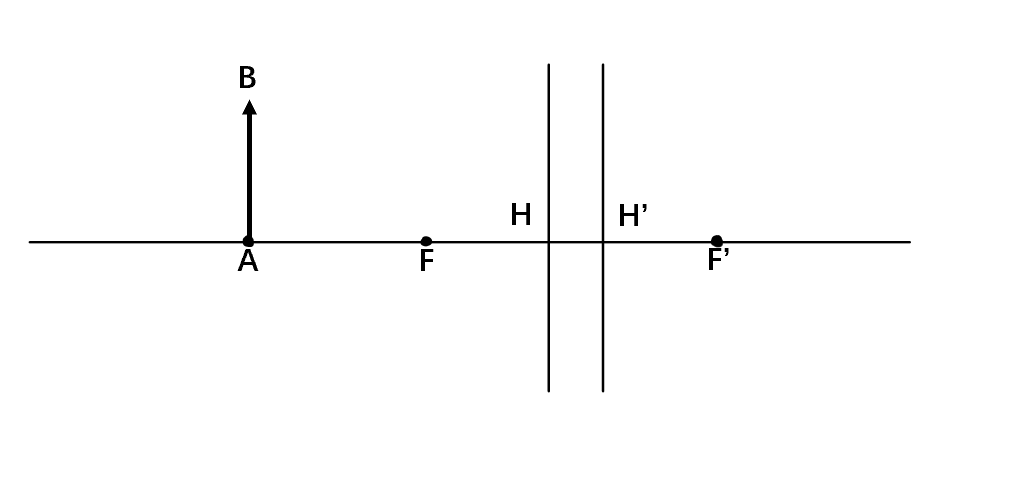
\includegraphics[scale=0.2]{1.png}% 插入图片,按50%的比例缩放
        \vspace{10mm}
        \item (2) 用作图法求下图薄透镜的焦点F, F'的位置。
         
        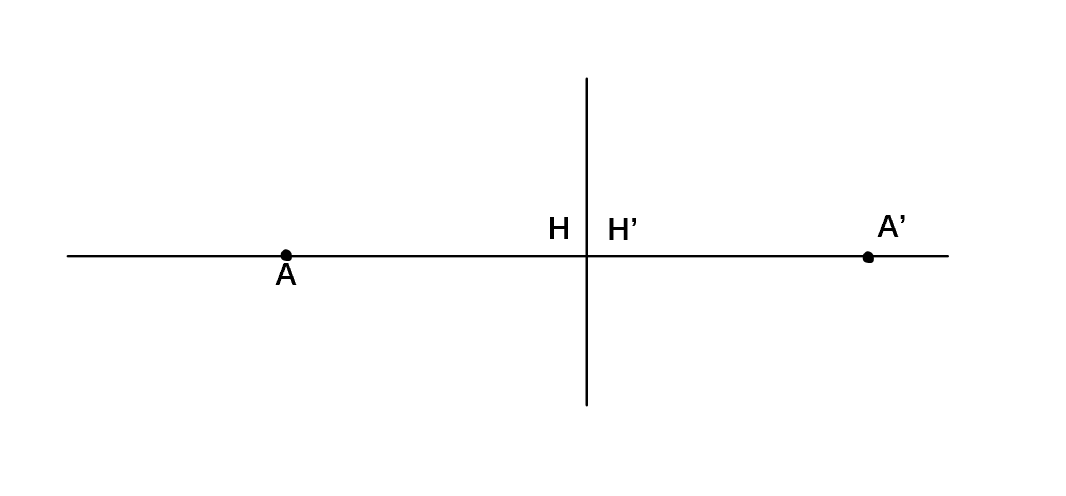
\includegraphics[scale=0.2]{2.png}% 插入图片,按50%的比例缩放
        \vspace{20mm}
        \item (3) 用作图法绘出下图薄透镜的焦点F,F'的位置(标在图上)
        
        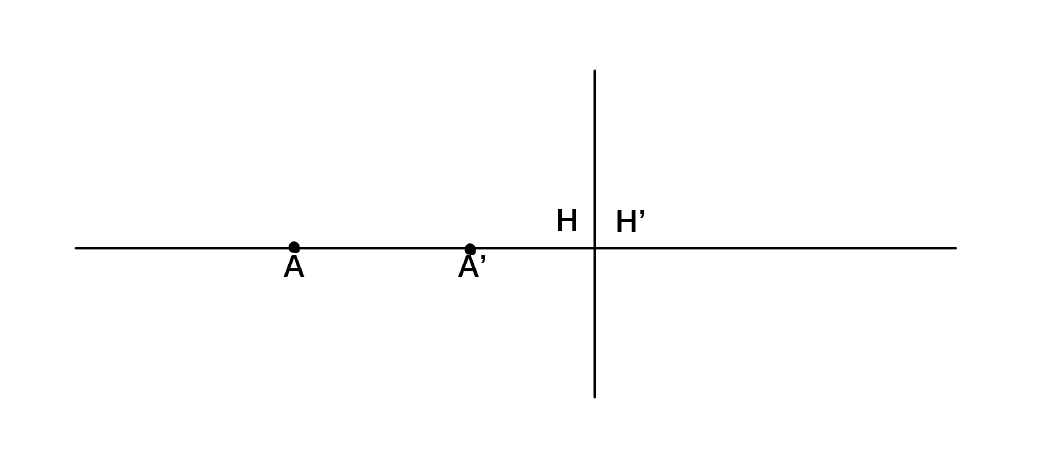
\includegraphics[scale=0.2]{3.png}% 插入图片,按50%的比例缩放
        \vspace{20mm}
        \item (4) 用作图法求图中垂轴像A'B'对应的物AB
        
        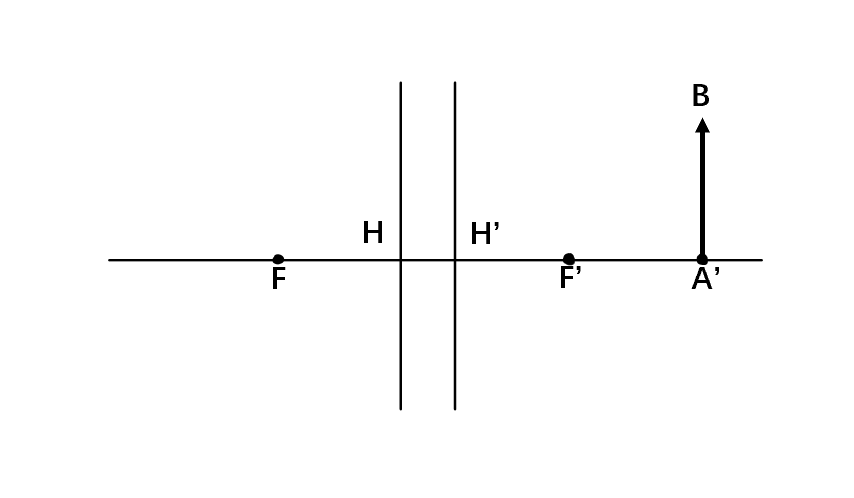
\includegraphics[scale=0.2]{4.png}% 插入图片,按50%的比例缩放
    \end{itemize}
    \section*{三、名词解释:本题共5小题。}
    \begin{enumerate}
        \vspace{0mm}
        \item 球差,位置色差,主点,节点,焦点,景深
        \vspace{0mm}
        \item 两束不同的激光能否发生干涉,请给出答案并说明理由
        \vspace{0mm}
        \item 自然双折射,感应双折射
        \vspace{0mm}
        \item 自然光变成线偏振光的四种方法
        \vspace{0mm}
        \item 一般性吸收,选择性吸收
    \end{enumerate}
    \section*{四、计算题:本题共5小题,顺序不确定}
    \subsection*{11.如图所示,光阑D位于薄透镜L左方30mm处,孔径为25mm,
    薄透镜焦距为60mm,直径40mm,物点A位于光阑左方120mm处.用计算法求轴上物点A的孔径光阑、入射光瞳、出射光瞳和视场光阑的位置和口径。}
    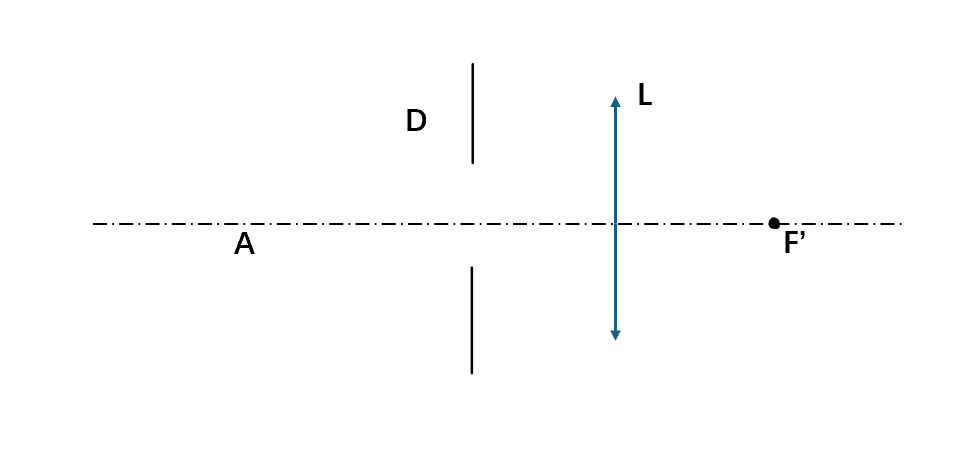
\includegraphics[scale=0.3]{5.png}
    \vspace{20mm}
    \subsection*{12.有一架开普勒望远镜,视放大率$\varGamma$ 为6,物方视场角$2\omega$ =$8\degree$,出瞳直径为$D'=5mm$,物镜和目镜之间的距离$L=140mm$,假定孔径光阑与物镜框重合,系统无渐晕,求:}
    \begin{itemize}
        \vspace{0mm}
        \item (1)物镜焦距\( f^{\prime} \)和目镜焦距\( f_{1}^{\prime} \)
        \vspace{0mm}
        \item (2)分划板直径:
        \vspace{0mm}
        \item (3)物镜口径\(\mathcal{D}_{\text{物}}\)和目镜口经\(\mathcal{D}_{\text{目}}\) 
        \vspace{0mm}
        \item (4)出瞳距离\(\mathcal{L}_{z}\)
    \end{itemize}
    \vspace{20mm}
    \subsection*{13.试确定下面两列光波的偏振状态,并给出归一化琼斯矢量形式}
    \begin{itemize}
        \vspace{0mm}
        \item \(E_{1}=A_{0}\left[e_{x}\cos (\omega t-kz)+e_{y}\cos (\omega t-kz-\frac{\pi}{2})\right] \)
        \item \(E_{2}=A_{0}\left[e_{x}\sin (\omega t-kz)+e_{y}\sin (\omega t-kz-\frac{\pi}{2})\right] \)
    \end{itemize}
    \vspace{20mm}
    \subsection*{14.如图所示,两相干平行光夹角为$\alpha $,在垂直于角平分线的方位上放置一观察屏,试确定观察屏上干涉条纹的形状及相邻亮条纹的间隔。}
    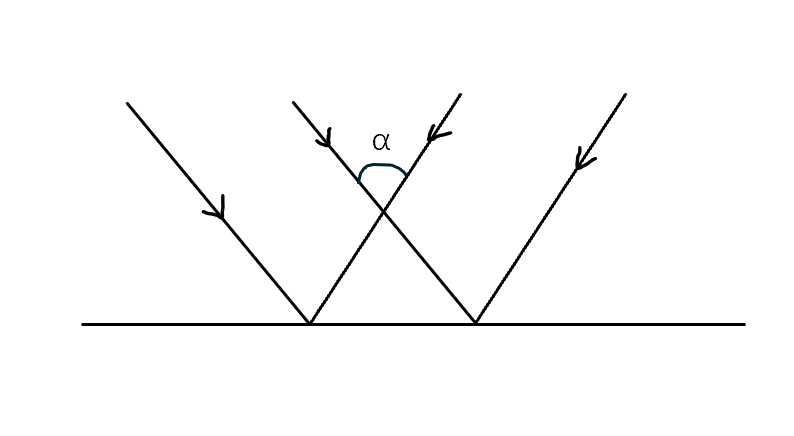
\includegraphics[scale=0.3]{6.png}
    \vspace{20mm}
    \subsection*{15.在杨氏双缝干涉实验装置中,双缝间隔为$0.5mm$,接收屏距双缝$1m$,点光源距离双缝$300mm$,发射出$500nm$的单色光,试求:}
    \begin{itemize}
        \vspace{-3mm}
        \item (1)屏上干涉条纹的间隔。
        \vspace{-3mm}
        \item (2)若点光源由光轴向下平移$2mm$,屏上干涉条纹向什么方向移动?移动多少距离?
        \vspace{-3mm}
        \item (3)若光源有一定的宽度,屏上干涉条纹消失时,它的临界宽度是多少?
    \end{itemize}
    \subsection*{16.一束自然光以布儒斯特角由空气入射到红宝石$(n=1.76)$表面上,试计算其表面反射率、透射率及反射光、透射光的偏振度。}
    \vspace{15mm}
    \subsection*{17.在双缝夫琅禾费衍射实验中,所用光波波长$\lambda =632.8nm$,透镜焦距$f=50cm$,观察到两相邻亮条纹之间的距离$e=1.5mm$,并且第4级亮纹缺级。\\试求:}
    \begin{itemize}
        \vspace{-3mm}
        \item (1)双缝的缝距和缝宽:
        \vspace{-3mm}
        \item (2)第1,2,3级亮纹的相对强度。
    \end{itemize}
    \vspace{15mm}
    \subsection*{18.一透镜的直径$D=2cm$,焦距$f=50cm$,受波长$\lambda =500nm$的平行光照射,试计算在该透镜焦平面上衍射图像的艾里斑大小。}
    \vspace{15mm}
    \subsection*{19.格兰-傅科(Glan-Foucault)棱镜\\方解石制成两个带有空气间隙的偏振棱镜,其中棱镜1的光轴垂直于入射面,光线按图示方向入射,已知\(n_{o}=1.658\),\(n_{e}=1.486\)。}
    \begin{itemize}
        \vspace{-3mm}
        \item (1) $\alpha $角在大于多少范围内,才能使入射的自然光经过棱镜后变为线偏振光。
        \vspace{-3mm}
        \item (2)若入射光强度相同,哪个棱镜的出射线偏振光更强?
        \vspace{-3mm}
        \item (3)画出自然光入射时的传输光路以及光的偏振状态。
        % 插入图片
    \end{itemize}
    \vspace{-3mm}
    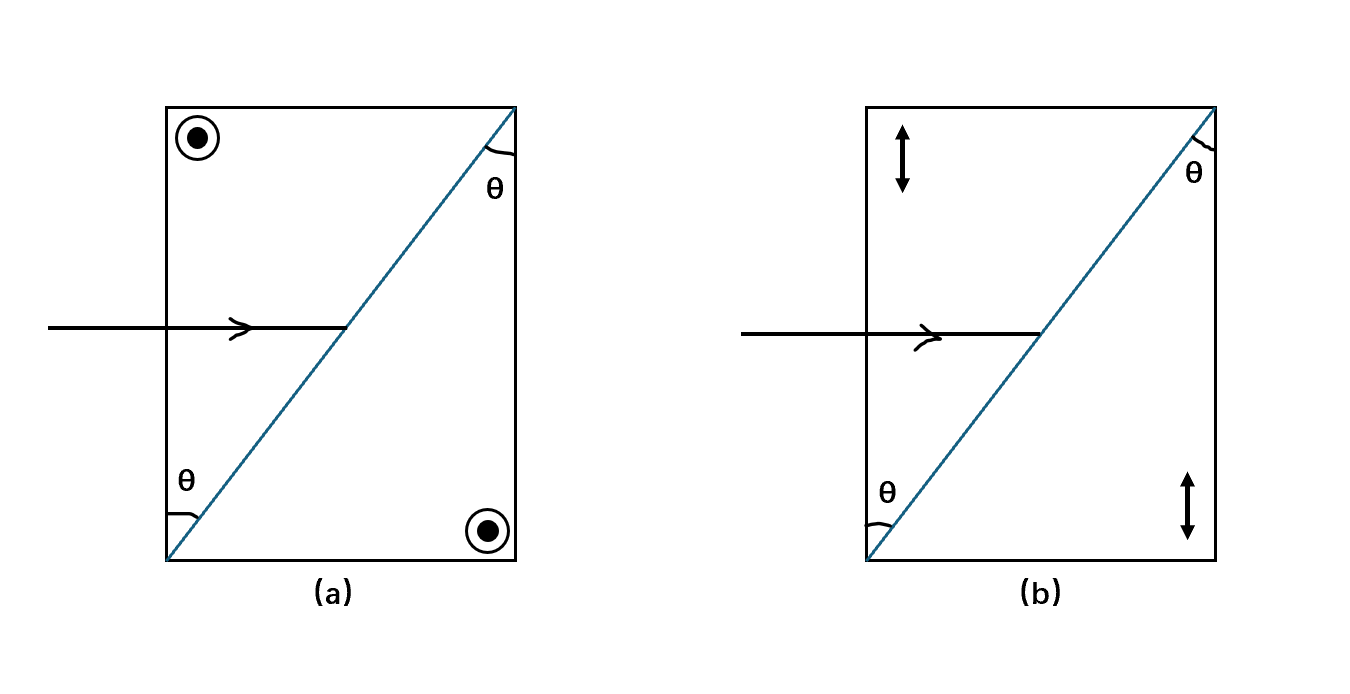
\includegraphics[scale=0.3]{7.png}
\end{document}